
%% bare_adv.tex
%% V1.4a
%% 2014/09/17
%% by Michael Shell
%% See: 
%% http://www.michaelshell.org/
%% for current contact information.
%%
%% This is a skeleton file demonstrating the advanced use of IEEEtran.cls
%% (requires IEEEtran.cls version 1.8a or later) with an IEEE Computer
%% Society journal paper.
%%
%% Support sites:
%% http://www.michaelshell.org/tex/ieeetran/
%% http://www.ctan.org/tex-archive/macros/latex/contrib/IEEEtran/
%% and
%% http://www.ieee.org/

%%*************************************************************************
%% Legal Notice:
%% This code is offered as-is without any warranty either expressed or
%% implied; without even the implied warranty of MERCHANTABILITY or
%% FITNESS FOR A PARTICULAR PURPOSE! 
%% User assumes all risk.
%% In no event shall IEEE or any contributor to this code be liable for
%% any damages or losses, including, but not limited to, incidental,
%% consequential, or any other damages, resulting from the use or misuse
%% of any information contained here.
%%
%% All comments are the opinions of their respective authors and are not
%% necessarily endorsed by the IEEE.
%%
%% This work is distributed under the LaTeX Project Public License (LPPL)
%% ( http://www.latex-project.org/ ) version 1.3, and may be freely used,
%% distributed and modified. A copy of the LPPL, version 1.3, is included
%% in the base LaTeX documentation of all distributions of LaTeX released
%% 2003/12/01 or later.
%% Retain all contribution notices and credits.
%% ** Modified files should be clearly indicated as such, including  **
%% ** renaming them and changing author support contact information. **
%%
%% File list of work: IEEEtran.cls, IEEEtran_HOWTO.pdf, bare_adv.tex,
%%                    bare_conf.tex, bare_jrnl.tex, bare_conf_compsoc.tex,
%%                    bare_jrnl_compsoc.tex, bare_jrnl_transmag.tex
%%*************************************************************************


% *** Authors should verify (and, if needed, correct) their LaTeX system  ***
% *** with the testflow diagnostic prior to trusting their LaTeX platform ***
% *** with production work. IEEE's font choices and paper sizes can       ***
% *** trigger bugs that do not appear when using other class files.       ***                          ***
% The testflow support page is at:
% http://www.michaelshell.org/tex/testflow/


% IEEEtran V1.7 and later provides for these CLASSINPUT macros to allow the
% user to reprogram some IEEEtran.cls defaults if needed. These settings
% override the internal defaults of IEEEtran.cls regardless of which class
% options are used. Do not use these unless you have good reason to do so as
% they can result in nonIEEE compliant documents. User beware. ;)
%
%\newcommand{\CLASSINPUTbaselinestretch}{1.0} % baselinestretch
%\newcommand{\CLASSINPUTinnersidemargin}{1in} % inner side margin
%\newcommand{\CLASSINPUToutersidemargin}{1in} % outer side margin
%\newcommand{\CLASSINPUTtoptextmargin}{1in}   % top text margin
%\newcommand{\CLASSINPUTbottomtextmargin}{1in}% bottom text margin




%
%\documentclass[10pt,journal,compsoc]{IEEEtran}
\documentclass[10pt,article]{IEEEtran}
% If IEEEtran.cls has not been installed into the LaTeX system files,
% manually specify the path to it like:
% \documentclass[10pt,journal,compsoc]{../sty/IEEEtran}


% For Computer Society journals, IEEEtran defaults to the use of 
% Palatino/Palladio as is done in IEEE Computer Society journals.
% To go back to Times Roman, you can use this code:
%\renewcommand{\rmdefault}{ptm}\selectfont





% Some very useful LaTeX packages include:
% (uncomment the ones you want to load)



% *** MISC UTILITY PACKAGES ***
%
%\usepackage{ifpdf}
% Heiko Oberdiek's ifpdf.sty is very useful if you need conditional
% compilation based on whether the output is pdf or dvi.
% usage:
% \ifpdf
%   % pdf code
% \else
%   % dvi code
% \fi
% The latest version of ifpdf.sty can be obtained from:
% http://www.ctan.org/tex-archive/macros/latex/contrib/oberdiek/
% Also, note that IEEEtran.cls V1.7 and later provides a builtin
% \ifCLASSINFOpdf conditional that works the same way.
% When switching from latex to pdflatex and vice-versa, the compiler may
% have to be run twice to clear warning/error messages.






% *** CITATION PACKAGES ***
%
\ifCLASSOPTIONcompsoc
  % IEEE Computer Society needs nocompress option
  % requires cite.sty v4.0 or later (November 2003)
  \usepackage[nocompress]{cite}
\else
  % normal IEEE
  \usepackage{cite}
\fi
% cite.sty was written by Donald Arseneau
% V1.6 and later of IEEEtran pre-defines the format of the cite.sty package
% \cite{} output to follow that of IEEE. Loading the cite package will
% result in citation numbers being automatically sorted and properly
% "compressed/ranged". e.g., [1], [9], [2], [7], [5], [6] without using
% cite.sty will become [1], [2], [5]--[7], [9] using cite.sty. cite.sty's
% \cite will automatically add leading space, if needed. Use cite.sty's
% noadjust option (cite.sty V3.8 and later) if you want to turn this off
% such as if a citation ever needs to be enclosed in parenthesis.
% cite.sty is already installed on most LaTeX systems. Be sure and use
% version 5.0 (2009-03-20) and later if using hyperref.sty.
% The latest version can be obtained at:
% http://www.ctan.org/tex-archive/macros/latex/contrib/cite/
% The documentation is contained in the cite.sty file itself.
%
% Note that some packages require special options to format as the Computer
% Society requires. In particular, Computer Society  papers do not use
% compressed citation ranges as is done in typical IEEE papers
% (e.g., [1]-[4]). Instead, they list every citation separately in order
% (e.g., [1], [2], [3], [4]). To get the latter we need to load the cite
% package with the nocompress option which is supported by cite.sty v4.0
% and later.





% *** GRAPHICS RELATED PACKAGES ***
%
\ifCLASSINFOpdf
  % \usepackage[pdftex]{graphicx}
  % declare the path(s) where your graphic files are
  % \graphicspath{{../pdf/}{../jpeg/}}
  % and their extensions so you won't have to specify these with
  % every instance of \includegraphics
  % \DeclareGraphicsExtensions{.pdf,.jpeg,.png}
\else
  % or other class option (dvipsone, dvipdf, if not using dvips). graphicx
  % will default to the driver specified in the system graphics.cfg if no
  % driver is specified.
  % \usepackage[dvips]{graphicx}
  % declare the path(s) where your graphic files are
  % \graphicspath{{../eps/}}
  % and their extensions so you won't have to specify these with
  % every instance of \includegraphics
  % \DeclareGraphicsExtensions{.eps}
\fi
% graphicx was written by David Carlisle and Sebastian Rahtz. It is
% required if you want graphics, photos, etc. graphicx.sty is already
% installed on most LaTeX systems. The latest version and documentation
% can be obtained at: 
% http://www.ctan.org/tex-archive/macros/latex/required/graphics/
% Another good source of documentation is "Using Imported Graphics in
% LaTeX2e" by Keith Reckdahl which can be found at:
% http://www.ctan.org/tex-archive/info/epslatex/
%
% latex, and pdflatex in dvi mode, support graphics in encapsulated
% postscript (.eps) format. pdflatex in pdf mode supports graphics
% in .pdf, .jpeg, .png and .mps (metapost) formats. Users should ensure
% that all non-photo figures use a vector format (.eps, .pdf, .mps) and
% not a bitmapped formats (.jpeg, .png). IEEE frowns on bitmapped formats
% which can result in "jaggedy"/blurry rendering of lines and letters as
% well as large increases in file sizes.
%
% You can find documentation about the pdfTeX application at:
% http://www.tug.org/applications/pdftex





% *** MATH PACKAGES ***
%
%\usepackage[cmex10]{amsmath}
% A popular package from the American Mathematical Society that provides
% many useful and powerful commands for dealing with mathematics. If using
% it, be sure to load this package with the cmex10 option to ensure that
% only type 1 fonts will utilized at all point sizes. Without this option,
% it is possible that some math symbols, particularly those within
% footnotes, will be rendered in bitmap form which will result in a
% document that can not be IEEE Xplore compliant!
%
% Also, note that the amsmath package sets \interdisplaylinepenalty to 10000
% thus preventing page breaks from occurring within multiline equations. Use:
%\interdisplaylinepenalty=2500
% after loading amsmath to restore such page breaks as IEEEtran.cls normally
% does. amsmath.sty is already installed on most LaTeX systems. The latest
% version and documentation can be obtained at:
% http://www.ctan.org/tex-archive/macros/latex/required/amslatex/math/





% *** SPECIALIZED LIST PACKAGES ***
%\usepackage{acronym}
% acronym.sty was written by Tobias Oetiker. This package provides tools for
% managing documents with large numbers of acronyms. (You don't *have* to
% use this package - unless you have a lot of acronyms, you may feel that
% such package management of them is bit of an overkill.)
% Do note that the acronym environment (which lists acronyms) will have a
% problem when used under IEEEtran.cls because acronym.sty relies on the
% description list environment - which IEEEtran.cls has customized for
% producing IEEE style lists. A workaround is to declared the longest
% label width via the IEEEtran.cls \IEEEiedlistdecl global control:
%
% \renewcommand{\IEEEiedlistdecl}{\IEEEsetlabelwidth{SONET}}
% \begin{acronym}
%
% \end{acronym}
% \renewcommand{\IEEEiedlistdecl}{\relax}% remember to reset \IEEEiedlistdecl
%
% instead of using the acronym environment's optional argument.
% The latest version and documentation can be obtained at:
% http://www.ctan.org/tex-archive/macros/latex/contrib/acronym/


%\usepackage{algorithmic}
% algorithmic.sty was written by Peter Williams and Rogerio Brito.
% This package provides an algorithmic environment fo describing algorithms.
% You can use the algorithmic environment in-text or within a figure
% environment to provide for a floating algorithm. Do NOT use the algorithm
% floating environment provided by algorithm.sty (by the same authors) or
% algorithm2e.sty (by Christophe Fiorio) as IEEE does not use dedicated
% algorithm float types and packages that provide these will not provide
% correct IEEE style captions. The latest version and documentation of
% algorithmic.sty can be obtained at:
% http://www.ctan.org/tex-archive/macros/latex/contrib/algorithms/
% There is also a support site at:
% http://algorithms.berlios.de/index.html
% Also of interest may be the (relatively newer and more customizable)
% algorithmicx.sty package by Szasz Janos:
% http://www.ctan.org/tex-archive/macros/latex/contrib/algorithmicx/




% *** ALIGNMENT PACKAGES ***
%
%\usepackage{array}
% Frank Mittelbach's and David Carlisle's array.sty patches and improves
% the standard LaTeX2e array and tabular environments to provide better
% appearance and additional user controls. As the default LaTeX2e table
% generation code is lacking to the point of almost being broken with
% respect to the quality of the end results, all users are strongly
% advised to use an enhanced (at the very least that provided by array.sty)
% set of table tools. array.sty is already installed on most systems. The
% latest version and documentation can be obtained at:
% http://www.ctan.org/tex-archive/macros/latex/required/tools/


%\usepackage{mdwmath}
%\usepackage{mdwtab}
% Also highly recommended is Mark Wooding's extremely powerful MDW tools,
% especially mdwmath.sty and mdwtab.sty which are used to format equations
% and tables, respectively. The MDWtools set is already installed on most
% LaTeX systems. The lastest version and documentation is available at:
% http://www.ctan.org/tex-archive/macros/latex/contrib/mdwtools/


% IEEEtran contains the IEEEeqnarray family of commands that can be used to
% generate multiline equations as well as matrices, tables, etc., of high
% quality.


%\usepackage{eqparbox}
% Also of notable interest is Scott Pakin's eqparbox package for creating
% (automatically sized) equal width boxes - aka "natural width parboxes".
% Available at:
% http://www.ctan.org/tex-archive/macros/latex/contrib/eqparbox/




% *** SUBFIGURE PACKAGES ***
%\ifCLASSOPTIONcompsoc
%  \usepackage[caption=false,font=footnotesize,labelfont=sf,textfont=sf]{subfig}
%\else
%  \usepackage[caption=false,font=footnotesize]{subfig}
%\fi
% subfig.sty, written by Steven Douglas Cochran, is the modern replacement
% for subfigure.sty, the latter of which is no longer maintained and is
% incompatible with some LaTeX packages including fixltx2e. However,
% subfig.sty requires and automatically loads Axel Sommerfeldt's caption.sty
% which will override IEEEtran.cls' handling of captions and this will result
% in non-IEEE style figure/table captions. To prevent this problem, be sure
% and invoke subfig.sty's "caption=false" package option (available since
% subfig.sty version 1.3, 2005/06/28) as this is will preserve IEEEtran.cls
% handling of captions.
% Note that the Computer Society format requires a sans serif font rather
% than the serif font used in traditional IEEE formatting and thus the need
% to invoke different subfig.sty package options depending on whether
% compsoc mode has been enabled.
%
% The latest version and documentation of subfig.sty can be obtained at:
% http://www.ctan.org/tex-archive/macros/latex/contrib/subfig/




% *** FLOAT PACKAGES ***
%
%\usepackage{fixltx2e}
% fixltx2e, the successor to the earlier fix2col.sty, was written by
% Frank Mittelbach and David Carlisle. This package corrects a few problems
% in the LaTeX2e kernel, the most notable of which is that in current
% LaTeX2e releases, the ordering of single and double column floats is not
% guaranteed to be preserved. Thus, an unpatched LaTeX2e can allow a
% single column figure to be placed prior to an earlier double column
% figure. The latest version and documentation can be found at:
% http://www.ctan.org/tex-archive/macros/latex/base/


%\usepackage{stfloats}
% stfloats.sty was written by Sigitas Tolusis. This package gives LaTeX2e
% the ability to do double column floats at the bottom of the page as well
% as the top. (e.g., "\begin{figure*}[!b]" is not normally possible in
% LaTeX2e). It also provides a command:
%\fnbelowfloat
% to enable the placement of footnotes below bottom floats (the standard
% LaTeX2e kernel puts them above bottom floats). This is an invasive package
% which rewrites many portions of the LaTeX2e float routines. It may not work
% with other packages that modify the LaTeX2e float routines. The latest
% version and documentation can be obtained at:
% http://www.ctan.org/tex-archive/macros/latex/contrib/sttools/
% Do not use the stfloats baselinefloat ability as IEEE does not allow
% \baselineskip to stretch. Authors submitting work to the IEEE should note
% that IEEE rarely uses double column equations and that authors should try
% to avoid such use. Do not be tempted to use the cuted.sty or midfloat.sty
% packages (also by Sigitas Tolusis) as IEEE does not format its papers in
% such ways.
% Do not attempt to use stfloats with fixltx2e as they are incompatible.
% Instead, use Morten Hogholm'a dblfloatfix which combines the features
% of both fixltx2e and stfloats:
%
% \usepackage{dblfloatfix}
% The latest version can be found at:
% http://www.ctan.org/tex-archive/macros/latex/contrib/dblfloatfix/


%\ifCLASSOPTIONcaptionsoff
%  \usepackage[nomarkers]{endfloat}
% \let\MYoriglatexcaption\caption
% \renewcommand{\caption}[2][\relax]{\MYoriglatexcaption[#2]{#2}}
%\fi
% endfloat.sty was written by James Darrell McCauley, Jeff Goldberg and 
% Axel Sommerfeldt. This package may be useful when used in conjunction with 
% IEEEtran.cls'  captionsoff option. Some IEEE journals/societies require that
% submissions have lists of figures/tables at the end of the paper and that
% figures/tables without any captions are placed on a page by themselves at
% the end of the document. If needed, the draftcls IEEEtran class option or
% \CLASSINPUTbaselinestretch interface can be used to increase the line
% spacing as well. Be sure and use the nomarkers option of endfloat to
% prevent endfloat from "marking" where the figures would have been placed
% in the text. The two hack lines of code above are a slight modification of
% that suggested by in the endfloat docs (section 8.4.1) to ensure that
% the full captions always appear in the list of figures/tables - even if
% the user used the short optional argument of \caption[]{}.
% IEEE papers do not typically make use of \caption[]'s optional argument,
% so this should not be an issue. A similar trick can be used to disable
% captions of packages such as subfig.sty that lack options to turn off
% the subcaptions:
% For subfig.sty:
% \let\MYorigsubfloat\subfloat
% \renewcommand{\subfloat}[2][\relax]{\MYorigsubfloat[]{#2}}
% However, the above trick will not work if both optional arguments of
% the \subfloat command are used. Furthermore, there needs to be a
% description of each subfigure *somewhere* and endfloat does not add
% subfigure captions to its list of figures. Thus, the best approach is to
% avoid the use of subfigure captions (many IEEE journals avoid them anyway)
% and instead reference/explain all the subfigures within the main caption.
% The latest version of endfloat.sty and its documentation can obtained at:
% http://www.ctan.org/tex-archive/macros/latex/contrib/endfloat/
%
% The IEEEtran \ifCLASSOPTIONcaptionsoff conditional can also be used
% later in the document, say, to conditionally put the References on a 
% page by themselves.





% *** PDF, URL AND HYPERLINK PACKAGES ***
%
%\usepackage{url}
% url.sty was written by Donald Arseneau. It provides better support for
% handling and breaking URLs. url.sty is already installed on most LaTeX
% systems. The latest version and documentation can be obtained at:
% http://www.ctan.org/tex-archive/macros/latex/contrib/url/
% Basically, \url{my_url_here}.


% NOTE: PDF thumbnail features are not required in IEEE papers
%       and their use requires extra complexity and work.
%\ifCLASSINFOpdf
%  \usepackage[pdftex]{thumbpdf}
%\else
%  \usepackage[dvips]{thumbpdf}
%\fi
% thumbpdf.sty and its companion Perl utility were written by Heiko Oberdiek.
% It allows the user a way to produce PDF documents that contain fancy
% thumbnail images of each of the pages (which tools like acrobat reader can
% utilize). This is possible even when using dvi->ps->pdf workflow if the
% correct thumbpdf driver options are used. thumbpdf.sty incorporates the
% file containing the PDF thumbnail information (filename.tpm is used with
% dvips, filename.tpt is used with pdftex, where filename is the base name of
% your tex document) into the final ps or pdf output document. An external
% utility, the thumbpdf *Perl script* is needed to make these .tpm or .tpt
% thumbnail files from a .ps or .pdf version of the document (which obviously
% does not yet contain pdf thumbnails). Thus, one does a:
% 
% thumbpdf filename.pdf 
%
% to make a filename.tpt, and:
%
% thumbpdf --mode dvips filename.ps
%
% to make a filename.tpm which will then be loaded into the document by
% thumbpdf.sty the NEXT time the document is compiled (by pdflatex or
% latex->dvips->ps2pdf). Users must be careful to regenerate the .tpt and/or
% .tpm files if the main document changes and then to recompile the
% document to incorporate the revised thumbnails to ensure that thumbnails
% match the actual pages. It is easy to forget to do this!
% 
% Unix systems come with a Perl interpreter. However, MS Windows users
% will usually have to install a Perl interpreter so that the thumbpdf
% script can be run. The Ghostscript PS/PDF interpreter is also required.
% See the thumbpdf docs for details. The latest version and documentation
% can be obtained at.
% http://www.ctan.org/tex-archive/support/thumbpdf/


% NOTE: PDF hyperlink and bookmark features are not required in IEEE
%       papers and their use requires extra complexity and work.
% *** IF USING HYPERREF BE SURE AND CHANGE THE EXAMPLE PDF ***
% *** TITLE/SUBJECT/AUTHOR/KEYWORDS INFO BELOW!!           ***
\newcommand\MYhyperrefoptions{bookmarks=true,bookmarksnumbered=true,
pdfpagemode={UseOutlines},plainpages=false,pdfpagelabels=true,
colorlinks=true,linkcolor={black},citecolor={black},urlcolor={black},
pdftitle={A Scale-first approach for Web API development},
pdfsubject={Typesetting},%<!CHANGE!
pdfauthor={Carlos Martin Flores G},
pdfkeywords={Computer Society, IEEEtran, journal, LaTeX, paper,
             template}}%<^!CHANGE!
%\ifCLASSINFOpdf
\usepackage[\MYhyperrefoptions,pdftex]{hyperref}
%\else
%\usepackage[\MYhyperrefoptions,breaklinks=true,dvips]{hyperref}
%\usepackage{breakurl}
%\fi
% One significant drawback of using hyperref under DVI output is that the
% LaTeX compiler cannot break URLs across lines or pages as can be done
% under pdfLaTeX's PDF output via the hyperref pdftex driver. This is
% probably the single most important capability distinction between the
% DVI and PDF output. Perhaps surprisingly, all the other PDF features
% (PDF bookmarks, thumbnails, etc.) can be preserved in
% .tex->.dvi->.ps->.pdf workflow if the respective packages/scripts are
% loaded/invoked with the correct driver options (dvips, etc.). 
% As most IEEE papers use URLs sparingly (mainly in the references), this
% may not be as big an issue as with other publications.
%
% That said, Vilar Camara Neto created his breakurl.sty package which
% permits hyperref to easily break URLs even in dvi mode.
% Note that breakurl, unlike most other packages, must be loaded
% AFTER hyperref. The latest version of breakurl and its documentation can
% be obtained at:
% http://www.ctan.org/tex-archive/macros/latex/contrib/breakurl/
% breakurl.sty is not for use under pdflatex pdf mode.
%
% The advanced features offer by hyperref.sty are not required for IEEE
% submission, so users should weigh these features against the added
% complexity of use.
% The package options above demonstrate how to enable PDF bookmarks
% (a type of table of contents viewable in Acrobat Reader) as well as
% PDF document information (title, subject, author and keywords) that is
% viewable in Acrobat reader's Document_Properties menu. PDF document
% information is also used extensively to automate the cataloging of PDF
% documents. The above set of options ensures that hyperlinks will not be
% colored in the text and thus will not be visible in the printed page,
% but will be active on "mouse over". USING COLORS OR OTHER HIGHLIGHTING
% OF HYPERLINKS CAN RESULT IN DOCUMENT REJECTION BY THE IEEE, especially if
% these appear on the "printed" page. IF IN DOUBT, ASK THE RELEVANT
% SUBMISSION EDITOR. You may need to add the option hypertexnames=false if
% you used duplicate equation numbers, etc., but this should not be needed
% in normal IEEE work.
% The latest version of hyperref and its documentation can be obtained at:
% http://www.ctan.org/tex-archive/macros/latex/contrib/hyperref/





% *** Do not adjust lengths that control margins, column widths, etc. ***
% *** Do not use packages that alter fonts (such as pslatex).         ***
% There should be no need to do such things with IEEEtran.cls V1.6 and later.
% (Unless specifically asked to do so by the journal or conference you plan
% to submit to, of course. )


% correct bad hyphenation here
\hyphenation{op-tical net-works semi-conduc-tor}
\usepackage[utf8]{inputenc}
\usepackage[english]{babel}
\usepackage[T1]{fontenc}
\usepackage{wrapfig}
\usepackage{epigraph}
\usepackage{caption}
\usepackage{graphicx}
\usepackage{framed}
\usepackage{hyperref}
\usepackage{longtable, multirow, booktabs}
\graphicspath{ {images/} }

\hypersetup{
    colorlinks=true,
    linkcolor=blue,
    filecolor=magenta,      
    urlcolor=cyan,
}

\urlstyle{same}

\begin{document}
%
% paper title
% Titles are generally capitalized except for words such as a, an, and, as,
% at, but, by, for, in, nor, of, on, or, the, to and up, which are usually
% not capitalized unless they are the first or last word of the title.
% Linebreaks \\ can be used within to get better formatting as desired.
% Do not put math or special symbols in the title.
\title{A Scale First approach for Web API development}
%
%
% author names and IEEE memberships
% note positions of commas and nonbreaking spaces ( ~ ) LaTeX will not break
% a structure at a ~ so this keeps an author's name from being broken across
% two lines.
% use \thanks{} to gain access to the first footnote area
% a separate \thanks must be used for each paragraph as LaTeX2e's \thanks
% was not built to handle multiple paragraphs
%
%
%\IEEEcompsocitemizethanks is a special \thanks that produces the bulleted
% lists the Computer Society journals use for "first footnote" author
% affiliations. Use \IEEEcompsocthanksitem which works much like \item
% for each affiliation group. When not in compsoc mode,
% \IEEEcompsocitemizethanks becomes like \thanks and
% \IEEEcompsocthanksitem becomes a line break with idention. This
% facilitates dual compilation, although admittedly the differences in the
% desired content of \author between the different types of papers makes a
% one-size-fits-all approach a daunting prospect. For instance, compsoc 
% journal papers have the author affiliations above the "Manuscript
% received ..."  text while in non-compsoc journals this is reversed. Sigh.


%\author{Carlos Mart\'{i}n Flores Gonz\'{a}lez \\ Costa Rica Institute of Technology ~\IEEEmembership{Student ID: 2015183528}}% <-this % stops a space

\author{\IEEEauthorblockN{Carlos Martín Flores González} \IEEEauthorblockA{School of Computer Engineering\\Costa Rica Institute of Technology\\Cartago, Costa Rica 2550--2254\\Email: \href{mailto:martin.flores@computer.org}{martin.flores@computer.org}\\
Student ID: 2015183528}}


% ======================================================

% \IEEEcompsocitemizethanks{\IEEEcompsocthanksitem M. Shell is with the Department
% of Electrical and Computer Engineering, Georgia Institute of Technology, Atlanta,
% GA, 30332.\protect\\
% note need leading \protect in front of \\ to get a newline within \thanks as
% \\ is fragile and will error, could use \hfil\break instead.
%E-mail: see http://www.michaelshell.org/contact.html
%\IEEEcompsocthanksitem J. Doe and J. Doe are with Anonymous University.}
%\thanks{Manuscript received April 19, 2005; revised September 17, 2014.}}

% ======================================================

% note the % following the last \IEEEmembership and also \thanks - 
% these prevent an unwanted space from occurring between the last author name
% and the end of the author line. i.e., if you had this:
% 
% \author{....lastname \thanks{...} \thanks{...} }
%                     ^------------^------------^----Do not want these spaces!
%
% a space would be appended to the last name and could cause every name on that
% line to be shifted left slightly. This is one of those "LaTeX things". For
% instance, "\textbf{A} \textbf{B}" will typeset as "A B" not "AB". To get
% "AB" then you have to do: "\textbf{A}\textbf{B}"
% \thanks is no different in this regard, so shield the last } of each \thanks
% that ends a line with a % and do not let a space in before the next \thanks.
% Spaces after \IEEEmembership other than the last one are OK (and needed) as
% you are supposed to have spaces between the names. For what it is worth,
% this is a minor point as most people would not even notice if the said evil
% space somehow managed to creep in.



% The paper headers
\markboth{Principles of Computer Science Research, August~2015}%
{Shell \MakeLowercase{\textit{et al.}}: Bare Advanced Demo of IEEEtran.cls for Journals}

% The only time the second header will appear is for the odd numbered pages
% after the title page when using the twoside option.
% 
% *** Note that you probably will NOT want to include the author's ***
% *** name in the headers of peer review papers.                   ***
% You can use \ifCLASSOPTIONpeerreview for conditional compilation here if
% you desire.



% The publisher's ID mark at the bottom of the page is less important with
% Computer Society journal papers as those publications place the marks
% outside of the main text columns and, therefore, unlike regular IEEE
% journals, the available text space is not reduced by their presence.
% If you want to put a publisher's ID mark on the page you can do it like
% this:
%\IEEEpubid{0000--0000/00\$00.00~\copyright~2014 IEEE}
% or like this to get the Computer Society new two part style.
%\IEEEpubid{\makebox[\columnwidth]{\hfill 0000--0000/00/\$00.00~\copyright~2014 IEEE}%
%\hspace{\columnsep}\makebox[\columnwidth]{Published by the IEEE Computer Society\hfill}}
% Remember, if you use this you must call \IEEEpubidadjcol in the second
% column for its text to clear the IEEEpubid mark (Computer Society journal
% papers don't need this extra clearance.)



% use for special paper notices
%\IEEEspecialpapernotice{(Invited Paper)}



% for Computer Society papers, we must declare the abstract and index terms
% PRIOR to the title within the \IEEEtitleabstractindextext IEEEtran
% command as these need to go into the title area created by \maketitle.
% As a general rule, do not put math, special symbols or citations
% in the abstract or keywords.
%\IEEEtitleabstractindextext{%

% Note that keywords are not normally used for peerreview papers.
%\begin{IEEEkeywords}
%Computer Society, IEEEtran, journal, \LaTeX, paper, template.
%\end{IEEEkeywords}}


% make the title area
\maketitle

\begin{abstract}
Most applications using the Web as a delivery mechanism have had to embrace practices in order to constantly adapt their software to ensure their applications will be up and running most of the time. This is not an easy task, and it becomes harder when applications are not designed to accommodate this change upfront.
Web Application Programming Interfaces (APIs) have become a popular solution to deliver data and content through the Web, and since they are available through the Internet, they are exposed to the same concerns on how to manage change, particularly the way the application can scale and manage new resources. Scale First is an attempt to describe an approach where scalability topics are placed first when implementing a Web API. It proposes a set of architectural, design and coding principles that allow addressing change more effectively. These principles can be used in conjunction with software development methodologies to model the system's strategy in terms of scalability and evolution.

\end{abstract}


% To allow for easy dual compilation without having to reenter the
% abstract/keywords data, the \IEEEtitleabstractindextext text will
% not be used in maketitle, but will appear (i.e., to be "transported")
% here as \IEEEdisplaynontitleabstractindextext when compsoc mode
% is not selected <OR> if conference mode is selected - because compsoc
% conference papers position the abstract like regular (non-compsoc)
% papers do!
\IEEEdisplaynontitleabstractindextext
% \IEEEdisplaynontitleabstractindextext has no effect when using
% compsoc under a non-conference mode.


% For peer review papers, you can put extra information on the cover
% page as needed:
% \ifCLASSOPTIONpeerreview
% \begin{center} \bfseries EDICS Category: 3-BBND \end{center}
% \fi
%
% For peerreview papers, this IEEEtran command inserts a page break and
% creates the second title. It will be ignored for other modes.
\IEEEpeerreviewmaketitle


\ifCLASSOPTIONcompsoc
\IEEEraisesectionheading{\section{Introduction}\label{sec:introduction}}
\else
\section{Introduction}
\label{sec:introduction}
\fi
% Computer Society journal (but not conference!) papers do something unusual
% with the very first section heading (almost always called "Introduction").
% They place it ABOVE the main text! IEEEtran.cls does not automatically do
% this for you, but you can achieve this effect with the provided
% \IEEEraisesectionheading{} command. Note the need to keep any \label that
% is to refer to the section immediately after \section in the above as
% \IEEEraisesectionheading puts \section within a raised box.




% The very first letter is a 2 line initial drop letter followed
% by the rest of the first word in caps (small caps for compsoc).
% 
% form to use if the first word consists of a single letter:
% \IEEEPARstart{A}{demo} file is ....
% 
% form to use if you need the single drop letter followed by
% normal text (unknown if ever used by IEEE):
% \IEEEPARstart{A}{}demo file is ....
% 
% Some journals put the first two words in caps:
% \IEEEPARstart{T}{his demo} file is ....
% 
% Here we have the typical use of a "T" for an initial drop letter
% and "HIS" in caps to complete the first word.
\IEEEPARstart{I}{n} software development, the use of APIs is crucial to define protocols, operations and tools for building applications. Software developers access APIs as interfaces for code libraries to speed up development and/or take advantage of existing low level tasks. With the advent of the World Wide Web, the most successful distributed system, a new kind of API has emerged in order to provide services in applications through a set of Hypertext Transfer Protocol (HTTP) messages, the Web API. But, as with APIs, most of today's Web APIs have a big problem: once deployed, they can't be changed. In fact, there are big-name APIs that stay static for years at a time, as the industry changes around them, because changing them would be too difficult\cite{RESTfulWebAPI:richardson}. A Web API's ability to adapt and evolve to new requirements is crucial to ensure its success under critical and high-demanding scenarios, such as the ones experienced by E-Commerce and data intensive applications.

 
\epigraph{{\textit{``Most software systems are created with the implicit assumption that the entire system is under the control of one entity, or at least that all entities participating within a system are acting towards a common goal and not at cross-purposes. Such an assumption cannot be safely made when the system runs openly on the Internet.''}}}{\textit{--- ~Roy Fielding \\ Architectural Styles and the Design of Network-based Software Architectures}}

Although we know software can change, many Web APIs can't accommodate change easily because they were not designed and developed with scalability in mind from the ground up. A scalable Web API is an application that has the ability not only to allocate new resources in order to support new demanding growth, but also to decrease resource consumption when demand is down. Scalability is one of the main concerns that organizations have to keep in mind when implementing a software project. Without it, the ability to compete and bring services to a broader audience, and even reputation, are compromised.


Software methodologies don't propose a specific set of actions to consider in order to address scalability concerns. Some agile methodologies such as Scrum and Extreme Programming (XP) encourage software projects to hit production or production-like environments as soon as possible (one of these approaches is the ``Walking Skeleton'', described by Allistair Cockburn\cite{cockburn} were a tiny implementation of the system is supposed to perform a small end-to-end function.) Their main goal is to quickly get feedback about the deployment process and minimize further risks. In this aspect, we can say that these methodologies are intended to model the domain of the application rather than application growth.

On the other hand, modern engineering practices such as Continuous Integration and Continuous Delivery provide us with a reference on how to manage applications, their changes in the codebase and their deployment. In both practices, automation emerges as one of the key aspects since they rely on software to run test $\to$ build $\to$ acceptance $\to$ deploy cycles\footnote{In Continuous Delivery, this workflow is known as a deployment pipeline.}; this could allow not only faster response times during deployment but also a better sense of quality\cite{humble}. In Continuous Delivery, the deployment processes of applications might consider scalability concerns because the goal is to model a workflow where applications are always in a delivery-ready state and, in order to achieve it, software developers have to find a way to provide mechanisms where applications are available to be shipped to one or \textit{n} servers at any time (ideally.)
An important thing to note here is that these practices are agnostic to the application they serve. This makes sense at first glance, but at the same time it could lead to scenarios where monolithic\footnote{The term monolith has been in use by the Unix community for some time. It appears in The \emph{Art of Unix Programming} to describe systems that get too big.} applications are trying to be deployed. Despite the success of monolithic applications, frustration increases especially when they are being deployed. Change cycles are tightly coupled, small changes require the entire monolith to be rebuilt and deployed. Over time it is often hard to keep a good modular structure, making it harder to keep changes that ought to only affect one module within that module. Scaling requires scaling of the entire application rather than parts of it that require greater resource\cite{monolit:fowler}. An application could be delivered fast, but its internals do not allow for a better way to scale it unless you try to scale the whole application at the same time. This approach could be expensive in terms of money as well as resource consumption. 

From the deployment standpoint, according to recent trends, organizations are planning for hybrid cloud computing solutions, meaning that they are increasingly relying their application deployment on more than one cloud computing provider\cite{rightscale}, making it even more important to have applications with cloud-friendly architectures. Here again, the eventual adoption of a development strategy that is aware of these kinds of deployment considerations could make application distribution easy and prevent further headaches.
 
% \hfill August 3, 2015

\section{Web APIs}
Web API is a term that refers to functions/operations that can be programmatically invoked using Web protocols. The term is based on the concept of Service Oriented Architecture (SOA) which proposed an attempt to change how software functionality is exposed through well-defined interfaces that were formally registered and could be discovered on the fly.

As the SOA notions matured, especially in their web services style and XML format of data, SOA evolved into more Web-friendly technologies such as Representational State Transfer (REST) and JSON data format that greatly simplified the reusability of an enterprise's capabilities. We use a common term, Web APIs, to refer to them.

The reason Web APIs are even more important today is that they allow organizations to make their business functionalities easily accessible  to  other  entities  (patterns,  customers)  and  thus  easily create new value-added services. Furthermore, users have more access than ever to a computing  device  in  the  context  of  their  daily  lives, i.e., mobiles.\cite{webapi:definition}

\section{Introducing Scale First}
Due the lack of a software methodology/approach that is able to embrace scalability concerns as a key role of the software development process of Web APIs from their initial designs, we introduce an approach where scalability becomes a feature of the application itself. By sticking to this approach, Web APIs will be able to evolve more easily because growth aspects are attacked in the initial stages of the development process, making organizations and individuals even more aware of the entire Web API ecosystem.

In order to have \textit{scale-ready} applications, Scale First proposes a set of principles for clean, well-structured and testable applications that will be able to evolve according their needs before a single line of code is written; here is where this approach differs from traditional methodologies, since concepts such as software design and deployment are tightly coupled. 

 
\subsection{Principles in Scale First}
\begin{itemize}
    \item Resizable deployment environments
    \item Technology agnostic design
    \item Modular, scalable application design
    \begin{itemize}
        \item Decompose application domain 
        \item Split conceptual model into separate models for update and display
    \end{itemize}
    \item Testability and maintainability
    \item Automated deployment process
    \item Define a scalability policy
\end{itemize}

\subsection{Resizable deployment environments}
Web APIs on \textit{Scale First} are intended to provide an elastic architecture. This requires a suitable deployment environment that provides support for this elastic behavior, since applications and their resources can change, so the goal here is to be ready to handle this change as fast as possible. This will increase Web APIs' availability and resilience. One popular alternative for providing a flexible environment for Web APIs is the adoption of cloud\footnote{The most-used definition of cloud computing belongs to the US National Institute of Standards and Technology (NIST): \textit{``Cloud computing is a model for enabling ubiquitous, convenient, on-demand network access to a shared pool of configurable computing resources (e.g. networks, servers, storage, applications and services) that can be rapidly provisioned and released with minimal management effort or service provider interaction\cite{nist:cloud-definition}''}} technologies. Software and infrastructure are increasingly consumed from the cloud. This is more flexible and much cheaper than deploying your own infrastructure, especially for smaller organizations.

Providers use three well-known models: IaaS (infrastructure as a service), PaaS (platform as a service) and SaaS (software as a service). As an example, in the case of IaaS, the model offers precise scalability. The cloud can outperform the physical hardware's classic scale-up or scale-out strategies. To gain as much from these features, applications have to be architected with as much as decoupling as possible, using SOA and queries between services.

\subsection{Technology agnostic design}
The aim of technology agnostic design(TAD) is to separate design and architecture from the technology employed and the specific implementation. This separation decreases both cost and risk while increasing scalability and availability of the Web API.
With TAD, both organizations and individuals are forced to create disciplines around scales that are not dependent on any single provider or service. This discipline allows you to scale in multiple dimensions through multiple potential partners, the result of which is a more predictable scalable system independent of any single solution provider. One popular option 

A common misperception is that by implementing a certain solution --for instance a database technology--, you are reliant on that solution. Just because the project makes use of a trendy new database technology does not mean that the Web API is dependent upon it alone for scale. TAD also impacts availability. The most obvious way is how it supports the ability to switch technology providers when one provider has significantly greater quality availability over another.

\subsubsection{TAD considerations for Web APIs} \cite{artofscalability} proposes three steps for TAD designs. These steps are suitable for Web API projects as well, and can act as an initial help guide.

\begin{enumerate}
    \item
    In the design itself, think in terms of boxes and wire diagrams rather than prose. Leave the detail of the boxes to the next step.
    \item
    In defining boxes and flows, use generic terms. Application server, Web server, RDBMS\footnote{RDBMS stands for \textit{Relational Database Management Systems}}, and so on. Don't use vendor names.
    \item
    Describe requirements in industry standards. Stay away from proprietary terms specific to a vendor.  
\end{enumerate}

If the design is being pulled toward a vendor in a description or design statement, try to ``loose'' that statement in order to make it agnostic.


  

 

% Although there are plenty of options for development and infrastructure for any Web API in mind, architecture is a design and should not rely upon any given vendor for implementation. 

\subsection{Modular, scalable application design}
Much has been written and implemented regarding the benefits of modular and/or component-based architectures in software development. These principles and practices apply to the development of Web APIs too, but beyond this, the goal is to come up with an architecture that allows the Web API to become an autonomous component that communicates with a mechanism such as web service requests, or remote procedure calls. That is, make the Web API a service\footnote{Or a \textit{microservice}, an architectural style to develop a single application as a suite of small services, each running in its own process and communicating with lightweight mechanisms, often an HTTP resource API\cite{monolit:fowler}. }.
From a scalability standpoint, the main reasons for using services as components are:
\begin{itemize}
    \item
    Technology Heterogeneity: Web APIs can be developed using the best suitable tool or technology stack depending on their needs.
    \item
    Only those services that need scaling will scale.
    \item
    Services are independently deployable: a change that is made to a single service is deployed  independently without impacting other systems. This allows for a faster deployment of the code. If a problem does occur, it can be isolated quickly to an individual service, making fast rollback easy to achieve.
    \item
    Resilience: working as an isolated service; if a Web API fails, that failure will not be propagated to other systems.
\end{itemize}

Notice the above are not the only characteristics of a service-oriented architecture. More of this is described in \cite{microservices} and \cite{monolit:fowler}. 

\subsubsection{Decompose application domain}
The domain context of the Web API must be clearly defined. The aim here is not to motivate the creation of very specific applications doing just one thing. This could lead to management issues, and since we are addressing the Web API development from a scalability standpoint, we are more interested in the creation of applications that represent a functional unit, so that logic and features inside can be managed and shared easily.

The work on \cite{evans:ddd} provides a guide on how to create systems that model real-world domains. It introduces the concept of \textit{bounded context}: ``a specific responsibility enforced by explicit boundaries''. The idea is that any given domain consists of multiple bounded contexts, and residing within each are things that do not need to be communicated to the outside, as well as things that are shared externally with other bounded contexts. Each bounded context has an explicit interface, where it decides what models to share with other contexts.
To get information from a bounded context, or if you want to make functionality requests within a bounded context, a communication with its explicit boundary using models is performed.

\begin{figure}[h]
    \hspace{-0.5cm}
    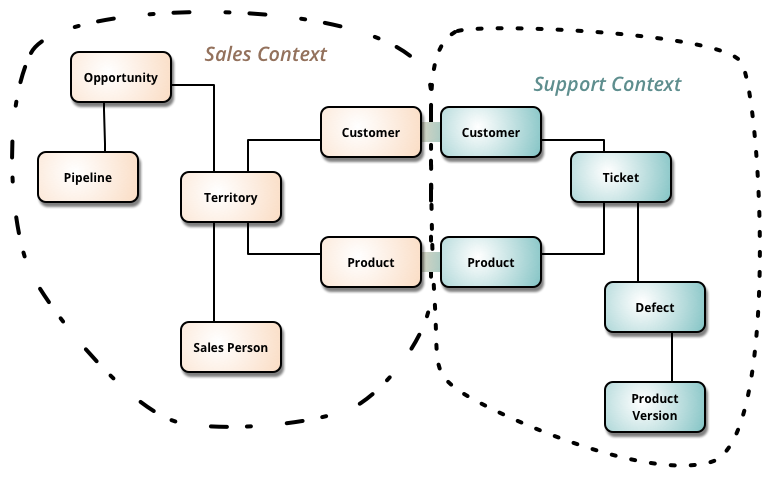
\includegraphics[width=9.5cm]{bounded-context}
    \caption{A fictional application domain with two bounded contexts: Sales Context and Support Context.\cite{fowler:bounded-context}}
    \label{fig:bounded-context}
\end{figure}


When developing a Web API, the domain can be separated into bounded contexts, meaning that each context has the potential to become a separate Web API. It doesn’t matter that the bounded contexts are not meant to be separate APIs in the initial stages of the Web API development process, because they can be extracted and implemented as separate APIs depending on the application’s needs.  This is why this separation process is crucial. With bounded contexts in place, future scalability efforts can be performed faster. This is therefore a very important activity to run when designing and developing applications that are meant to be subject of change. In the fictional application design on figure \ref{fig:bounded-context}, although a Web API can be developed using the entire domain as a reference, both Sales Context and Support Context are potential separate Web APIs. 

\subsubsection{Split conceptual model into separate models for update and display}
Depending on the domain, some applications can be more intensive in reading (query) than in writing data and vice versa.  Even so, both responsibilities have to be identified and separated into models for update and display. Ideally, each model will hold a set of autonomous components(such as databases) so each model is not depending on the other. This separation allows applications to scale based on the demand of each of its responsibilities; that way, if the most intensive part in a Web API is related to the query of data sources for display purposes, then this portion of the Web API can be isolated and segregated in another Web API whose only purpose will be to serve queries. Since queries are now being performed off of a separate data store from the master database, and assuming that the data that's being served is not 100\% up to date, one can easily add more instances of these stores without having to worry that they don’t contain the same exact data. This provides cheap horizontal scaling for queries. Also, since you are not doing nearly as much data transformation, the latency per query goes down as well. Simple code is fast code\cite{dahan:cqrs}.

An often implemented solution to this is the three-tiered application, which has a separate data, logic and presentation tier. Within this solution, the database in the data tier is often seen as one CRUD (Create, Read, Update and Delete data) data store in which all commands and queries are performed on the same database. This can lead to locking, performance and scalability problems, especially with larger commands or queries, since all things have to be taken care of sequentially. Distributing parts of the system in combination with selective locking of data provides a partial solution, but leads to a high probability of data inconsistency.
An option is to split parts of the system that have an emphasis on consistency from parts that should have an emphasis on availability or partition tolerance. The Command Query Responsibility Segregation (CQRS) is a pattern in which all logic in a software product is separated based on whether it changes the application state (commands) or only queries it (queries). This means that executing commands is done by components different from the one responsible for executing the querying tasks, all of which can be done distributed and in parallel.
Besides helping to solve the scalability problem of multi-tiered software products by enabling architects to distribute tasks of the system among an unlimited number of systems, CQRS also helps to implement a higher level of variability in online software products. The high level of variability is caused by the fact that the main pattern keeps commands strictly separated from queries and has a large collection of sub patterns using the distributed nature of the pattern to enable, among others, all sorts of tenant-dependent configurations, work flows, and business rules\cite{cqrs:kabbedijk}.

\begin{figure}[h]
    \centering
    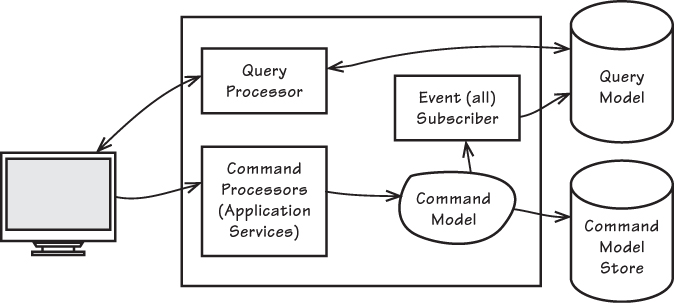
\includegraphics[width=9cm]{cqrs}
    \caption{With CQRS, commands from clients travel one way to the command model. Queries are run against a separate data source optimized for presentation and delivered as user interface or reports\cite{vernon:iddd}.}
    \label{fig:cqrs}
\end{figure}

With a CQRS approach like the one in figure \ref{fig:cqrs} one can lead a Web API to be separated in two subapplications, each application can grow independently so resources can be assigned depending on its demand. 

\subsection{Testability and maintainability}
A test strategy for a Web API that is intended to evolve quickly must provide the following:
\begin{enumerate}
    \item
    Tests must run fast
    \item
    Tests must cover as much of the application as possible
    \item
    Tests must be automated
    \item
    Continuous Integration
\end{enumerate}

In the above list, items 1, 2 and 3 are intended to describe how a test should behave while item 4 is intended to provide a context for how tests should be executed. Although many kinds of testing exist\cite{humble}, testing for fast and reliable scaling must have the automated component. For Web APIs, unit, integration and acceptance tests are the preferable set of tests to include.

The idea behind item 4, continuous integration, is that if regular integration of your codebase is good, why not do it all the time? In the context of integration, ``all the time'' means every single time somebody adds a change into the system\cite{beck:ci}. The application of this concept in the Web API by the usage of continuous integration software\footnote{Jenkins, Bamboo, Cruise Control, SnapCI, TravisCI} in the development process will allow delivering software much faster, and with fewer bugs\footnote{Or with no bugs at all}. 


To increase the Web API autonomy and increase overall availability, it is also necessary to identify and repair problems, and then notify the appropriate system operator of the service's current status. A Web API must provide support to actively monitor its internal state, act on potential trouble, try to heal itself, and continuously publish its status. For this, \cite{soapatterns} proposes the implementation of a service watchdog\footnote{\textit{Watchdog} is a term borrowed from the embedded systems world. A watchdog is a hardware device that counts down to 0, at which point it takes action, such as resetting the device. To prevent this reset, the application has to ``kick the dog'' before the timer runs out. If the application doesn't reset the counter, it could mean that the application has stopped responding. A reset would fix that.}, a pattern where a service actively monitors its internal state, acts on potential trouble, tries to heal itself, and continuously publishes its status. Web APIs on \textit{Scale First} must contain a component in charge of monitoring the API's state. This component publishes the API's state periodically, and also when something meaningful occurs.

%The Service Watchdog pattern (see figure 3.14) revolves around a single idea—you%can increase the service’s responsibility by combining two complementary concepts:%reporting and self-healing.
%The first is the watchdog agent concept, where the service implements the Active%Service pattern (discussed in chapter 2) and contains a component in charge of monitoring%the service’s state. This component publishes the service’s state periodically,%and also when something meaningful occurs



\subsection{Automated deployment process}
\textit{Scale First} relies on the concepts and principles behind Continuous Delivery\cite{humble} in order to define processes that will allow having a Web API application in a delivery-ready state. To achieve this, continuous delivery introduces the concept of \textit{deployment pipeline} which is an automated manifestation of the process for getting software from version control to the users. Every change in the software goes through a complex process on its way to being released. That process involves the building of the software, followed by the progress of these builds through multiple stages of testing and deployment. The deployment pipeline models this process, and its incarnation in a continuous integration and release management tool is what allows seeing and controlling the progress of each change as it moves from version control through various sets of tests and deployment to release to users. %A figure representing a basic pipeline can be found in appendix \ref{sec:deployment-pipeline}.

An automated deployment process for a Web API in \textit{Scale First} must include tasks in which new resources are able to be both, allocated and deallocated according to application demands. This ability to make applications and environments adjust to new conditions is what we refer to as the \textit{scale-ready} attribute in this Web API development approach. 
 

\subsection{Define a scalability policy}
As with every new paradigm, it's important to design Web APIs taking into account best practices and policies that will act as a body of knowledge for the application.
The definition of policies and practices on \textit{Scale First} must cover:
\begin{itemize}
    \item
    Design for failure
    \item
    High availability
    \item
    Performance
    \item
    Security
    \item
    Monitoring
\end{itemize}

\subsubsection{Design for failure}
High scalability has limitations. Redundancy and fault tolerance are primary design goals. Applications have  to be prepared for reboots and launches.

\subsubsection{High availability}
IT resource disruption has a huge negative impact on any business, this leads to design with outages and high availability in mind.

\subsubsection{Performance}
It is necessary to consider technology limitations regarding performance. A usage burst can affect available resources, notably compute units and disks' input/output operations. Bottlenecks might arise as a result of latency issues. 

\subsubsection{Security}
Enforce well-established security practices around the Web API: firewalls, minimal server services to reduce attack vectors, up-to-date operating systems, key-based authentication, and so on.

\subsubsection{Monitoring}
The ease of deployment of new resources can make the number of servers grow exponentially. This raises new issues, and monitoring tools are vital to system management.


\subsection{Web API Checklist on Scale First}

\newcommand{\ra}[1]{\renewcommand{\arraystretch}{#1}}
\begin{table}[h!]
    \ra{0.98}
    \centering
    \begin{tabular}{lc|c} 
        \toprule[1.5pt]
        & \multicolumn{2}{c}{\textbf{Implemented?}} \\
        \textbf{Feature} & \textbf{Yes} & \textbf{No} \\ \hline
        \emph{Infrastructure} & & \\
        \hspace{0.2cm}Infrastructure is flexible?  & & \\
        \emph{Application Domain} & & \\
        \hspace{0.2cm}Domain is delimited &  & \\
        \hspace{0.2cm}Display (Quey) model &  & \\
        \hspace{0.2cm}Update (Command) model & & \\
        \emph{Test Strategy} & & \\
        \hspace{0.2cm}Unit Tests & & \\
        \hspace{0.2cm}Integration Tests & & \\
        \hspace{0.2cm}Acceptance Tests & & \\
        \hspace{0.2cm}Continuous Integration software & &\\
        Automated deployment & & \\
        \hspace{0.2cm}Deployment pipeline is defined? & &\\ 
        \emph{Policies} & & \\
        \hspace{0.2cm}Failure& & \\
        \hspace{0.2cm}High Availability & & \\
        \hspace{0.2cm}Performance & & \\
        \hspace{0.2cm}Security & & \\
        \hspace{0.2cm}Monitoring & &\\                 
    \bottomrule[1.5pt]
    \end{tabular}
    \caption{Web API Checklist on Scale First}\label{table:checklist}    
\end{table}


\ifCLASSOPTIONcompsoc
    \IEEEraisesectionheading{\section{Experimental Setup}\label{sec:experimental}}
\else
    \section{Experimental Setup}
\label{sec:experimentals}
\fi

The exploratory study of the impact of the \textit{Scale First} approach for Web API development could be composed of four parts. In the first part we can collect a set of Web API projects in which one or more of the principles of the Scale First approach have not been adopted. In the second part, the development of a non-trivial Web API that follows the \textit{Scale First} approach is required. This allow us to identify the potential of \textit{Scale First}. In the third part, we need to create and perform scenarios where scalability is required on both types of applications: those that follow \textit{Scale First} and those that don't. Lastly, we measure and interpret the impact of Scale First by analyzing the response time involved in performing the scalability task and the resources assigned to it, such as money, hardware and people.


\subsection{First part: Web APIs don't follow Scale First principles}
This experiment involves the gathering of Web API projects where some of the \textit{Scale First} principles are not adopted. For starters, classic monolithical (``three tier'') applications could be the target. These applications could be architected taking some, but not all, of the exposed principles into account. 

\subsection{Second part: Development of a non-trivial Web API following Scale First principles}
A Web API project following the \textit{Scale First} principles must be developed. Ideally this should be a project that will be used in a real-life scenario. It could mimic the size and complexity of one of the applications gathered in the first part. Another interesting approach would be to perform a migration project of one of the applications in the first part to the \textit{Scale First} model.

\subsection{Third part: Evaluation}
In this part of the experiment we need to create and perform tests in which both types of applications need to react to change in some way. Some initial scenarios could involve:

\begin{itemize}
    \item
    Scale a new instance of the Web API to a new server.
    \item
    Scale a new instance of the Web API into a new cloud provider.
    \item
    Once a new instance of the Web API is deployed, terminate it.
    \item
    Extract a portion of an existing Web API to an independent Web API.
    \item
    Add a new resource to the application (database, cache, third party solution)
\end{itemize}

The above list proposes some basic scenarios where scalability concerns are tested. Depending on the nature of the application and organization needs, these scenarios could be more and could include more complex specifications.

\subsection{Fourth part: analysis and interpretation}
Once we have selected a set of Web APIs, is time to measure, analyze and interpret the data we obtained from the previous part. The goal here is to evaluate whether the adoption of the \textit{Scale First} principles in the development of the Web API causes a beneficial impact in comparison to the Web APIs that don't follow this approach.

Here, it is very important to select the most relevant metrics and then ask questions about the impact of those metrics in the scale process of a Web API:
\begin{itemize}
    \item
    How much time does the scale process take?
    \item
    How many people were involved in the process?
    \item
    What was the user feedback (if any)?
    \item
    How much money is needed to scale the Web API resources?
    \item
    Which cloud provider has better response time?
    \item
    How were the memory consumption or disks' input/output operations impacted? 
\end{itemize}



% needed in second column of first page if using \IEEEpubid
%\IEEEpubidadjcol

%\subsubsection{Subsubsection Heading Here}
%Subsubsection text here.


% An example of a floating figure using the graphicx package.
% Note that \label must occur AFTER (or within) \caption.
% For figures, \caption should occur after the \includegraphics.
% Note that IEEEtran v1.7 and later has special internal code that
% is designed to preserve the operation of \label within \caption
% even when the captionsoff option is in effect. However, because
% of issues like this, it may be the safest practice to put all your
% \label just after \caption rather than within \caption{}.
%
% Reminder: the "draftcls" or "draftclsnofoot", not "draft", class
% option should be used if it is desired that the figures are to be
% displayed while in draft mode.
%
%\begin{figure}[!t]
%\centering
%\includegraphics[width=2.5in]{myfigure}
% where an .eps filename suffix will be assumed under latex, 
% and a .pdf suffix will be assumed for pdflatex; or what has been declared
% via \DeclareGraphicsExtensions.
%\caption{Simulation results for the network.}
%\label{fig_sim}
%\end{figure}

% Note that IEEE typically puts floats only at the top, even when this
% results in a large percentage of a column being occupied by floats.
% However, the Computer Society has been known to put floats at the bottom.


% An example of a double column floating figure using two subfigures.
% (The subfig.sty package must be loaded for this to work.)
% The subfigure \label commands are set within each subfloat command,
% and the \label for the overall figure must come after \caption.
% \hfil is used as a separator to get equal spacing.
% Watch out that the combined width of all the subfigures on a 
% line do not exceed the text width or a line break will occur.
%
%\begin{figure*}[!t]
%\centering
%\subfloat[Case I]{\includegraphics[width=2.5in]{box}%
%\label{fig_first_case}}
%\hfil
%\subfloat[Case II]{\includegraphics[width=2.5in]{box}%
%\label{fig_second_case}}
%\caption{Simulation results for the network.}
%\label{fig_sim}
%\end{figure*}
%
% Note that often IEEE papers with subfigures do not employ subfigure
% captions (using the optional argument to \subfloat[]), but instead will
% reference/describe all of them (a), (b), etc., within the main caption.
% Be aware that for subfig.sty to generate the (a), (b), etc., subfigure
% labels, the optional argument to \subfloat must be present. If a
% subcaption is not desired, just leave its contents blank,
% e.g., \subfloat[].


% An example of a floating table. Note that, for IEEE style tables, the
% \caption command should come BEFORE the table and, given that table
% captions serve much like titles, are usually capitalized except for words
% such as a, an, and, as, at, but, by, for, in, nor, of, on, or, the, to
% and up, which are usually not capitalized unless they are the first or
% last word of the caption. Table text will default to \footnotesize as
% IEEE normally uses this smaller font for tables.
% The \label must come after \caption as always.
%
%\begin{table}[!t]
%% increase table row spacing, adjust to taste
%\renewcommand{\arraystretch}{1.3}
% if using array.sty, it might be a good idea to tweak the value of
% \extrarowheight as needed to properly center the text within the cells
%\caption{An Example of a Table}
%\label{table_example}
%\centering
%% Some packages, such as MDW tools, offer better commands for making tables
%% than the plain LaTeX2e tabular which is used here.
%\begin{tabular}{|c||c|}
%\hline
%One & Two\\
%\hline
%Three & Four\\
%\hline
%\end{tabular}
%\end{table}


% Note that the IEEE does not put floats in the very first column
% - or typically anywhere on the first page for that matter. Also,
% in-text middle ("here") positioning is typically not used, but it
% is allowed and encouraged for Computer Society conferences (but
% not Computer Society journals). Most IEEE journals/conferences use
% top floats exclusively. 
% Note that, LaTeX2e, unlike IEEE journals/conferences, places
% footnotes above bottom floats. This can be corrected via the
% \fnbelowfloat command of the stfloats package.




\section{Conclusion}
This paper proposes a development approach for Web APIs and creates an experimental setup. This proposal takes into consideration the constantly-changing environment in which Web APIs live, and then exposes a set of alternatives to make these kinds of applications more adaptive. This is achieved by putting together patterns and practices that already exist in software development, but are not part of a single body of knowledge for the context of Web APIs.

Today Web APIs are everywhere. They act as backing services behind desktop, mobile and Web applications, which is why these development efforts are more important than ever.  \textit{Scale First} is an attempt to address Web API software development from a scalability standpoint. And, although we are just scratching the surface regarding the eventual benefits of this approach, we see a lot of potential in it in comparison with current and old methodologies and approaches to create software for the Web.




% if have a single appendix:
%\appendix[Proof of the Zonklar Equations]
% or
%\appendix  % for no appendix heading
% do not use \section anymore after \appendix, only \section*
% is possibly needed

% use appendices with more than one appendix
% then use \section to start each appendix
% you must declare a \section before using any
% \subsection or using \label (\appendices by itself
% starts a section numbered zero.)
%


%\appendices
%\section{A basic deployment pipeline}
%\label{sec:deployment-pipeline}
%
%\begin{figure*}[h]
%    \centering
%    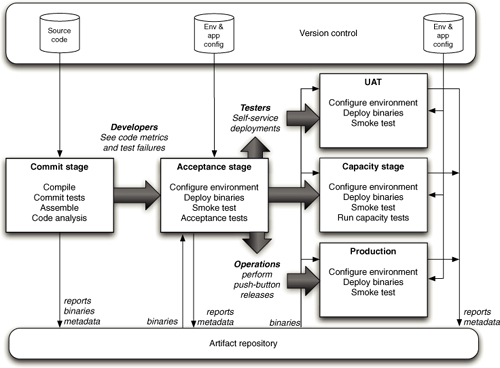
\includegraphics[width=12cm]{deployment-pipeline}
%    \caption{A basic deployment pipeline}
%    \label{fig:deployment-pipeline}
%\end{figure*}

%Appendix one text goes here.

% you can choose not to have a title for an appendix
% if you want by leaving the argument blank
%\section{}
%Appendix two text goes here.


% use section* for acknowledgment
%\ifCLASSOPTIONcompsoc
  % The Computer Society usually uses the plural form
%  \section*{Acknowledgments}
%\else
  % regular IEEE prefers the singular form
%  \section*{Acknowledgment}
%\fi


%The authors would like to thank...


% Can use something like this to put references on a page
% by themselves when using endfloat and the captionsoff option.
\ifCLASSOPTIONcaptionsoff
  \newpage
\fi



% trigger a \newpage just before the given reference
% number - used to balance the columns on the last page
% adjust value as needed - may need to be readjusted if
% the document is modified later
%\IEEEtriggeratref{8}
% The "triggered" command can be changed if desired:
%\IEEEtriggercmd{\enlargethispage{-5in}}

% references section

% can use a bibliography generated by BibTeX as a .bbl file
% BibTeX documentation can be easily obtained at:
% http://www.ctan.org/tex-archive/biblio/bibtex/contrib/doc/
% The IEEEtran BibTeX style support page is at:
% http://www.michaelshell.org/tex/ieeetran/bibtex/
%\bibliographystyle{IEEEtran}
% argument is your BibTeX string definitions and bibliography database(s)
%\bibliography{IEEEabrv,../bib/paper}
%
% <OR> manually copy in the resultant .bbl file
% set second argument of \begin to the number of references
% (used to reserve space for the reference number labels box)
\begin{thebibliography}{1}

\bibitem{artofscalability}
M.~Abbot and M.~Fisher, \emph{The art of scalability: scalable web architecture, processes, and organizations for the modern enterprise}, 1st~ed. Massachusetts, United States: Person Education, 2010.
  
\bibitem{scalabilityrules}
M.~Abbot and M.~Fisher, \emph{Scalability Rules: 50 Principles for Scaling Web Sites}, 1st~ed. Massachusetts, United States: Person Education, 2011.

\bibitem{beck:ci}
K.~Beck and C.~Andres. \emph{Extreme Programming Explained: Embrace Change.} 2nd edition, Addison-Wesley, 2004.

\bibitem{isw:cd}
L.~Chen, \emph{Continuous Delivery: Huge Benefits, but Challenges Too}, IEEE Software, vol. 32, no 2, 2015, pp. 50-54.

\bibitem{cockburn}
A.~Cockburn, \emph{Walking skeleton}. Available at: \url{http://alistair.cockburn.us/Walking+skeleton}

\bibitem{dahan:cqrs}
U.~Dahan. \emph{Clarified CQRS}. December, 2009. Available at: \href{http://udidahan.com/2009/12/09/clarified-cqrs/}{http://udidahan.com/2009/12/09/clarified-cqrs/}

\bibitem{growingpains}
E.~Espinha, A~Zaidman and HG~Gross \emph{Web API Growing Pains: Stories from Client Developers and Their Code}, Delf University of Technology, The Netherlands. 2014

\bibitem{evans:ddd}
E.~Evans. \emph{Domain-Driven Design}. Addison-Wesley. 2003.

\bibitem{fowler:bounded-context}
M.~Fowler. \emph{BoundedContext}. January, 2014. Available at: \href{http://martinfowler.com/bliki/BoundedContext.html}{http://martinfowler.com/bliki/BoundedContext.html}

\bibitem{monolit:fowler}
M.~Fowler, \emph{Microservices}. Available at: \url{http://martinfowler.com/articles/microservices.html}

\bibitem{humble}
J.~Humble and D.~Farley, \emph{Continuous delivery : reliable software releases through build, test, and deployment automation}, 1st~ed. Massachusetts, United States: Person Education, 2011.

\bibitem{cqrs:kabbedijk}
J.~Kabbedijk and S.~Jansen and S.~Brinkkemper. \emph{A Case Study of the Variability Consequences of the CQRS Pattern in Online Business Software}. Proceedings of the 17th European Conference on Pattern Languages of Programs. 2012.

\bibitem{nist:cloud-definition}
P.~Mell and T.~Grance. \emph{The NIST Definition of Cloud Computing}. US Nat'l Institute of Standards and Technology. 2011.

\bibitem{microservices}
S.~Newman, \emph{Building Microservices}, 1st~ed. O'Reilly Media Inc, 2015

\bibitem{RESTfulWebAPI:richardson}
L.~Richardson and M.~Amundsen, \emph{RESTful Web APIs}, 1st ~ed.\hskip 1em plus
  0.5em minus 0.4em\relax California, United States: O'Reilly Media Inc, 2013.

\bibitem{rightscale}
RightScale. \emph{RightScale 2015 State of the Cloud Report}. RightScale, Inc. 2005. Available at: \href{http://www.rightscale.com/lp/2015-state-of-the-cloud-report?campaign=701700000012UP6}{http://www.rightscale.com/lp/2015-state-of-the-cloud-report?campaign=701700000012UP6}

\bibitem{soapatterns}
A.~Rotem-Gal-Oz. \emph{SOA Patterns}. 1st ed. Manning Publications. 2012.

\bibitem{isw:cloud}
N.~Serrano, G. Gallardo and J.~Hernantes, \emph{Infrastructure as a Service and Cloud Technologies}, IEEE Software, vol. 32, no 2, 2015, pp. 30-36.

\bibitem{oscon:1}
T.~Schlossnagle, \emph{Scalable Internet Architectures}, O'Reilly Open Source Convention 2010. O'Reilly Media Inc, 2010.

\bibitem{webapi:definition}
B.~Srivastrava. \emph{Composing Web APIs: State of the Art and Mobile Implications (Tutorial)}. Proceeding MOBILESoft 2014 Proceedings of the 1st International Conference on Mobile Software Engineering and Systems. 2014.

\bibitem{vernon:iddd}
V.~Vernon. \emph{Implementing Domain Driven Design}. 1st ed. Addison-Wesley. July, 2013.


  
%\bibitem{IEEEhowto:kopka}
%H.~Kopka and P.~W. Daly, \emph{A Guide to {\LaTeX}}, 3rd~ed.\hskip 1em plus
%  0.5em minus 0.4em\relax Harlow, England: Addison-Wesley, 1999.
  
  
    

\end{thebibliography}

% biography section
% 
% If you have an EPS/PDF photo (graphicx package needed) extra braces are
% needed around the contents of the optional argument to biography to prevent
% the LaTeX parser from getting confused when it sees the complicated
% \includegraphics command within an optional argument. (You could create
% your own custom macro containing the \includegraphics command to make things
% simpler here.)
%\begin{IEEEbiography}[{\includegraphics[width=1in,height=1.25in,clip,keepaspectratio]{mshell}}]{Michael Shell}
% or if you just want to reserve a space for a photo:

%\begin{IEEEbiography}{Michael Shell}
%Biography text here.
%\end{IEEEbiography}


% You can push biographies down or up by placing
% a \vfill before or after them. The appropriate
% use of \vfill depends on what kind of text is
% on the last page and whether or not the columns
% are being equalized.

%\vfill

% Can be used to pull up biographies so that the bottom of the last one
% is flush with the other column.
%\enlargethispage{-5in}



% that's all folks
\end{document}


